

\subsection{Разработка структуры компонента для сбора информации}

В данном разделе будет детально рассмотрена структура модуля, его функции и алгорритмы функционирования. В разделе описываются компоненты, из которых состоих сам модуль, а так же связь между ними.


\subsubsection{Определение ключевых функций}

Разрабатываемый модуль состоит из трех компонентов. Рассмотрим функционал каждого подробнее.

\paragraph{Сбор и обработка данных}

Модуль должен быть способен автоматически собирать опросные данные с заполненных анкет посетителей парковки.

Был определен ряд вопросов, который позволяют определить некоторые основные интересы:
\begin{itemize}
    \item ­интересуетесь ли вы искусством (картины, скульптура, музыка и т.д.);
    \item ­занимаетесь ли вы спортом или физической активностью;
    \item ­любите ли вы чтение книг или просмотр фильмов;
    \item ­интересуетесь ли вы наукой и технологиями;
    \item ­увлекаетесь ли вы путешествиями и открытием новых мест;
    \item ­является ли для вас кулинария или готовка хобби;
    \item ­интересуетесь ли вы политикой и общественными вопросами.
\end{itemize}

Так же на бланке (представлен на рисунке~\ref{f:blank} выше) присутствует поле, в котором опрашиваемый должен указать свой возраст. 

Опрашиваемый должен закрасить кружки, соответствующие его ответу на каждый вопрос, а также указать свой возраст.

Бланк на вход должен подаваться в виде фотографии или скан копии.

Присутсвует возможность изменить блнак. Вопросы пользователь может выбрать произвольно, главное, чтобы они были представленны в определенном в примере формате. Для изменения областей интересов, с которыми работает система, необходимо внести их списком в текстовый файл. Далее система будет подгружать их в таблицу. Сам файл хранится в папке конфигурации по пути \textbackslash cfg от корневой папки и выглядит следущим образом (пример файла привен на рисунке~\ref{f:file-cfg}).

\begin{figure}[ht]
	\centering
	\vspace{\toppaddingoffigure}
	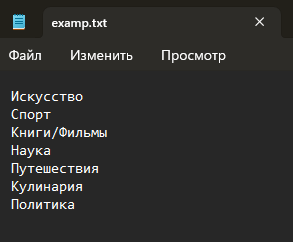
\includegraphics[width=0.45\textwidth]{file-cfg}
	\caption{Пример файла с конфигурацией областей интересов}
	\label{f:file-cfg}
\end{figure}

После сбора данных необходимо провести их предварительную обработку, включая распознавание текста и извлечение ответов на вопросы опроса.


\paragraph{­Распознавание номеров автомобилей}

Модуль должен обеспечивать распознавание номеров автомобилей с изображений, полученных с камер видеонаблюдения на парковке.

Разрешение входного изображения должно быть не ниже 1280х720. Кроме того, распознаваемый номер должен быть читаем, то есть быть чистым, не выцветшим и не закрыт посторонними предметами. Это позволит повысить точность распознавания и сократить количество ошибок.

После распознавания номеров необходимо извлечь информацию о модели автомобиля и ассоциировать её с данными о посетителе.

\paragraph{Поиск модели автомобиля}

Данный модуль должен по распознанному номеру найти модель автомобиля. Данная процедура должна выполнятся с помощью сторонних сервисов, например "Номерограмм.ру", которые позволяют получить базовую информации об автомобиле, на основе WIN-номера или гос. регистрационного знака.



\subsubsection{Структура модуля}

Необходимо сформировать наиболее точное описание разрабатываемого программного обеспечения. Для этого было принято решение о рассмотрении функциональной диаграммы верхнего уровня.

В данном случае в качестве отображения взаимосвязей была выбрана нотация IDEF0. В качестве входных бланк опроса и изображение автомобиля. В качестве субъекта выступает пользователь и вычислительная машина. Управление задается алгоритмами анализа бланков, распознавания номера и получения модели автомобиля. К выходным данным будут относиться информация об интересах посетителя, его возраст и модель машины.
Контекстная диаграмма IDEF0 представлена на рисунке~\ref{f:getdate_struct}.

\begin{figure}[ht]
	\centering
	\vspace{\toppaddingoffigure}
	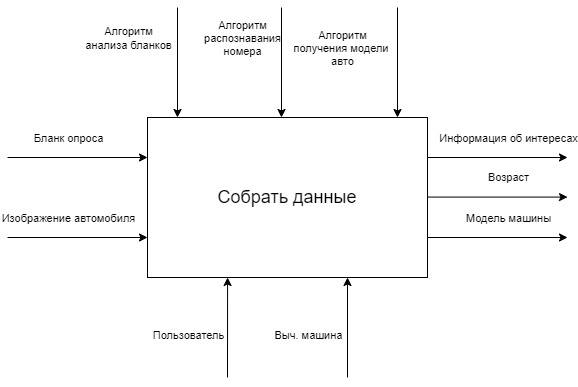
\includegraphics[width=0.7\textwidth]{getdate_struct}
	\caption{Контекстная диаграмма IDEF0}
	\label{f:getdate_struct}
\end{figure}

Детализирующая функциональная диаграмма более подробно раскрывает функциональную диаграмму верхнего уровня: описывает взаимодействия и связи процессов, происходящих внутри системы. На ней можно увидеть, какие процессы взаимосвязаны и что между ними общего.
На детализирующей функциональной диаграмме показаны следующие этапы:

\begin{itemize}
    \item анализ бланков. Входными данными являются бланки опросов. На выход поступает информация об интересах и возраст опрашиваемого;
    \item­ распознавание номеров. Входными данными являются изображения автомобилей. На выход поступает государственный номер автомобиля;
    \item­ определение модели. На вход поступает номер автомобиля, а на выход идет модель машины.
\end{itemize}

Детализированная контекстная диаграмма представлена на рисунке~\ref{f:getdate_struct_det}.
\begin{figure}[ht]
	\centering
	\vspace{\toppaddingoffigure}
	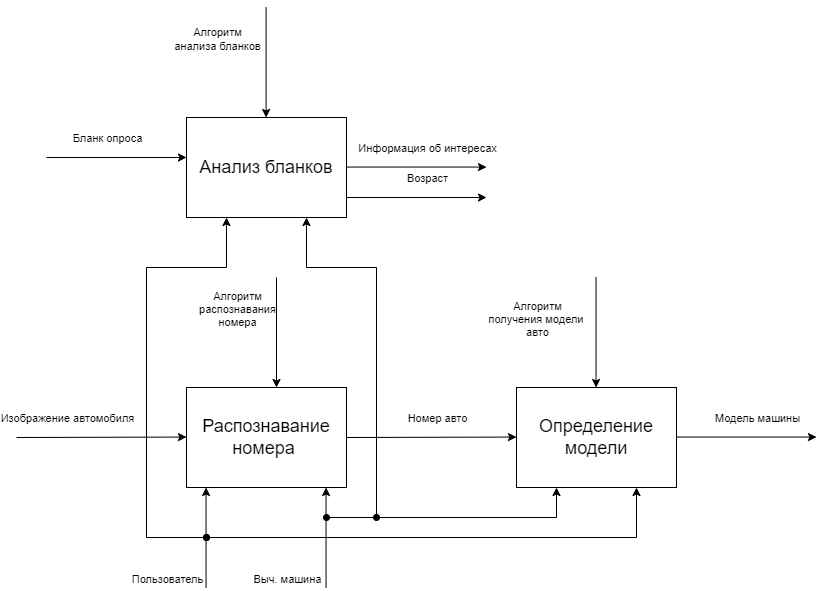
\includegraphics[width=0.7\textwidth]{getdate_struct_det}
	\caption{Детализированная контекстная диаграмма IDEF0}
	\label{f:getdate_struct_det}
\end{figure}

Таким образом, разрабатываемый модуль будет состоять из трех основных компонентов: «Анализ бланков», «Определение модели», «Распознавание номера».

Так же стоит определить формат создаваемого датасета. В него будет входить вся получаемая информация. Следовательно, датасет будет иметь следующие поля:

\begin{itemize}
    \item model: модель автомобиля;
    \item age: возраст;
    \item art: интерес к искусству;
    \item sport: интерес к спорту;
    \item book/film: интерес к фильмам и книгам;
    \item science: интерес к науке и технологиям;
    \item travel: интерес к путешествиям;
    \item cooking: интерес к готовке;
    \item politics: интерес к политике.
\end{itemize}


\subsubsection{Анализатор бланков}

Основными функциями компонента являются функции для анализа анкет, сбора информации об ответах и возрасте, указанном на бланке.

Задача компонента заключается в анализе анкет. Он должен автоматически обрабатывать изображения анкет, извлекать информацию об ответах на вопросы и возрасте, указанном на бланке.

Для выполнения задачи выбраны следующие инструменты:
\begin{itemize}
    \item OpenCV: для обработки изображений, выделения контуров и преобразований перспективы;
    \item imutils: для удобной работы с изображениями, сортировки контуров и других операций;
    \item pytesseract: для распознавания текста на изображениях с использованием технологии OCR.
\end{itemize}

На вход компоненту подается изображение анкеты. Это может быть фотография сверху или скан копия бланка. После своей работы результаты будут сохраняются в CSV-файл.

Рассмотрим алгоритм работы компонента:
\begin{enumerate}
    \item начало: вход в компонент;
    \item ­загрузка изображения: компонент получает на вход изображение анкеты для анализа;
    \item ­препроцессинг изображения;
        \begin{enumerate}
            \item преобразование в оттенки серого;
            \item сглаживание с помощью фильтра Гаусса;
            \item применение оператора Canny для обнаружения границ;
        \end{enumerate}
    \item ­поиск области анкеты;
        \begin{enumerate}
            \item поиск контуров на изображении;
            \item определение контура анкеты;
        \end{enumerate}
    \item выделение области анкеты;
        \begin{enumerate}
            \item применение преобразования перспективы для выделения области анкеты;
            \item получение и сохранение выделенной области;
        \end{enumerate}
    \item обработка анкеты;
        \begin{enumerate}
            \item применение пороговой обработки к выделенной области для получения четкого изображения;
            \item обнаружение контуров на обработанном изображении;
            \item определение контуров блоков с ответами на анкете;
        \end{enumerate}
    \item анализ ответов;
        \begin{enumerate}
            \item идентификация блоков с ответами на анкете;
            \item определение заполненных ответов в каждом блоке;
            \item оценка правильности ответов согласно ключу ответов;
            \item формирование списка результатов анализа;
        \end{enumerate}
    \item извлечение возраста;
        \begin{enumerate}
            \item определение области, содержащей возраст на анкете;
            \item применение преобразования перспективы для выделения области с возрастом;
            \item применение пороговой обработки и распознавание текста для извлечения возраста;
        \end{enumerate}
    \item запись результатов: сохранение результатов анализа и возраста в файл;
    \item конец: завершенеи работы компонента.
\end{enumerate}

Алгоритм работы компонента представлен на рисунке~\ref{f:blank_alg}.
\begin{figure}[ht]
	\centering
	\vspace{\toppaddingoffigure}
	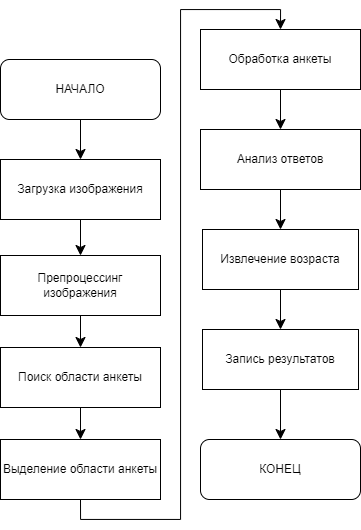
\includegraphics[width=0.4\textwidth]{blank_alg}
	\caption{Алгоритм работы анализатора}
	\label{f:blank_alg}
\end{figure}

Данный модуль в принципе является самостоятельным. Он может использоваться в различных областях, где требуется автоматизированный анализ анкет. Также при желании, его можно расширить и настроить для анализа других типов анкет.

Также не стоит забывать об обработке ошибок. При реализации данного компонента необходимо предусмотреть решение ошибочных ситуаций (неправильное распознавание, неверный формат изображения), которые могут возникать в процессе работы, чтобы обеспечить корректную работу.


\subsubsection{Поиск модели автомобиля}

Разработку компонента стоит начать с определения основной функции: обеспечение автоматизированного доступа к информации о моделях автомобилей. Информацию о модели можно взять с различных сайтов, таких как Nomerogram.ru, Avtocod.ru и другие. Важно учесть, что работа с сайтом будет вестись программно, а значит стоит выбрать сайт не только с самой большой базой автомобилей, но и тот, у которого нет «проверки на робота». Из представленных вариантов, а именно Nomerogram.ru, Avtocod.ru, Autoteka.ru, Avtoproverka.ru, имеющих примерно одинаковую базу автомобилей, все кроме Autoteka.ru имеют так называемую «проверку на робота» (рисунок~\ref{f:check_robot}).

\begin{figure}[ht]
	\centering
	\vspace{\toppaddingoffigure}
	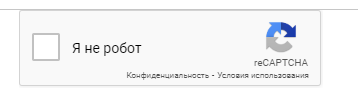
\includegraphics[width=0.4\textwidth]{check_robot}
	\caption{Проверка на робота}
	\label{f:check_robot}
\end{figure}


Следовательно, работа будет происходить именно с Autoteka.ru (рисунок~\ref{f:autoteka}).

\begin{figure}[ht]
	\centering
	\vspace{\toppaddingoffigure}
	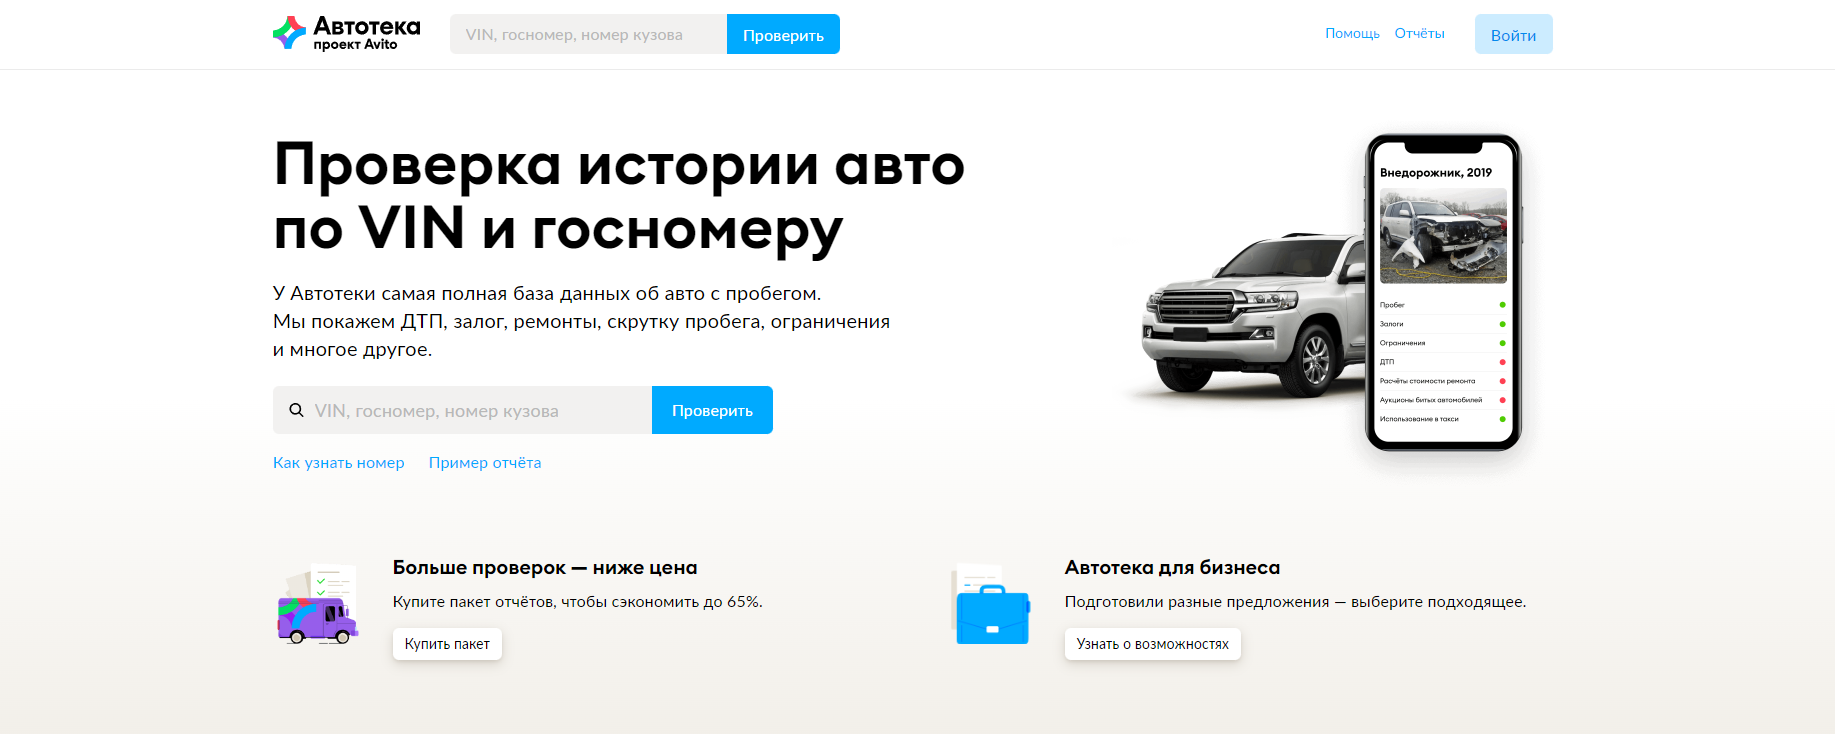
\includegraphics[width=0.85\textwidth]{autoteka}
	\caption{Главный экран Autoteka.ru}
	\label{f:autoteka}
\end{figure}

Autoteka.ru – это веб-сервис, который собирает и предоставляет информацию о различных транспортных средствах на территории России. Он пользуется популярностью среди водителей, автодилеров, страховых компаний и других участников автомобильного сектора. Вот основные характеристики и особенности сайта autoteka.ru:

\begin{itemize}
    \item проверка истории автомобиля. На сайте autoteka.ru пользователи могут проверить историю определенного автомобиля, используя его номер регистрации. Эта функция предоставляет информацию о предыдущих владельцах, результатах технического осмотра, наличии ограничений на регистрацию, участии в ДТП и других значимых данных;
    \item получение технических данных. Люди могут просматривать информацию о технических характеристиках машины, таких как бренд, модель, год выпуска, тип кузова, мощность двигателя и других деталях. Это может быть полезно при принятии решения о покупке или продаже автомобиля;
    \item проверка наличия ограничений. Пользователи имеют возможность проверить, есть ли какие-либо ограничения на регистрацию автомобиля, такие как залоги, аресты или запреты на регистрацию по различным причинам. Это важно для тех, кто планирует приобрести автомобиль, и желает удостовериться в его юридической чистоте перед сделкой;
    \item получение отчетов по автомобилю. Пользователи имеют возможность запросить подробные отчеты об истории автомобиля, включая информацию о предыдущих сделках, количестве владельцев, технических характеристиках, участии в ДТП и прочих данных. Это способствует осознанному выбору при покупке подержанного транспортного средства;
    \item онлайн-консультации. Кроме того, на avtoteka.ru доступны онлайн-консультации и помощь пользователям по вопросам автомобильной истории, юридическим аспектам регистрации транспортных средств и другим темам.
\end{itemize}



Avtoteka.ru – это востребованный ресурс среди пользователей, источник полезной информации о транспортных средствах. С его помощью можно узнать всё, что важно о машине, просто введя VIN-код, госномер или номер кузова. Процесс простой: вводите данные и жмёте "Поиск", после чего получаете страницу с информацией о транспортном средстве (рисунок~\ref{f:autoteka_info}).

\begin{figure}[ht]
	\centering
	\vspace{\toppaddingoffigure}
	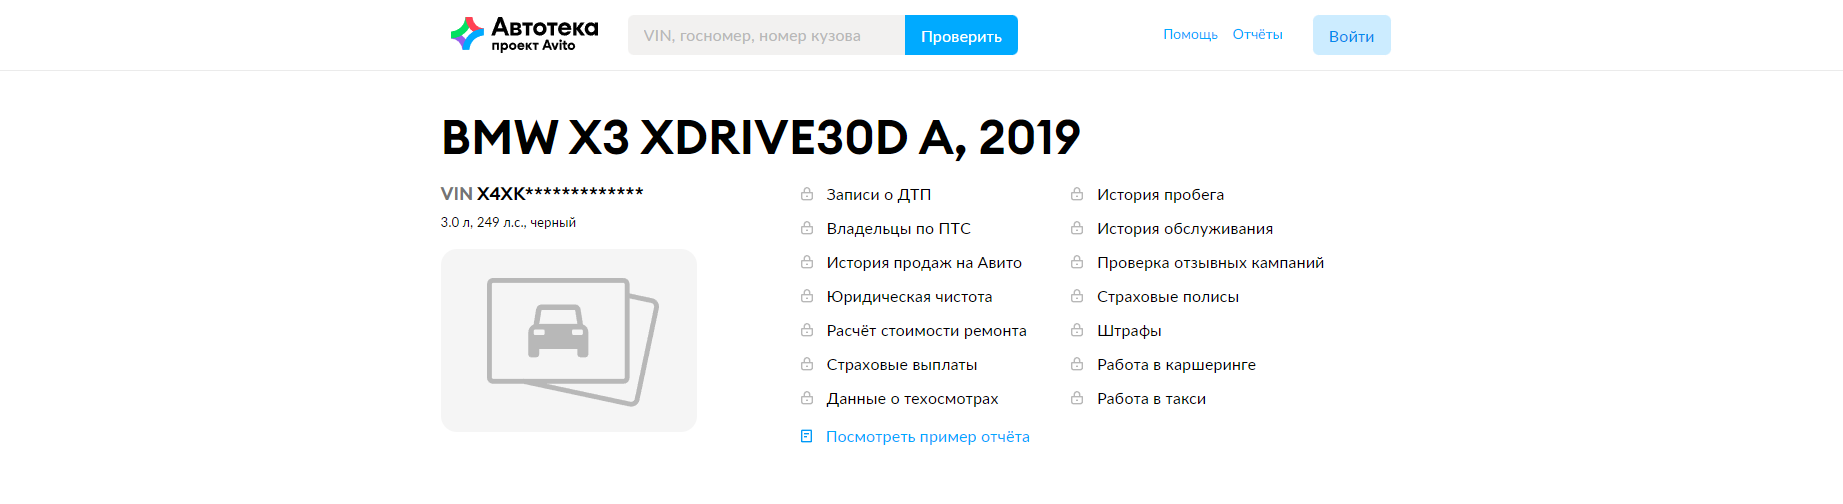
\includegraphics[width=1\textwidth]{autoteka_info}
	\caption{Информация об автомобиле}
	\label{f:autoteka_info}
\end{figure}

Полная информация предоставляется по платной подписке или за разовый платеж, но для выполнения поставленной задачи необходимо получить только модель, что можно сделать бесплатно.


Функциональные требования: компонент должен обеспечивать ввод номера, отправку запроса на сайт Autoteka, получение результатов и извлечение необходимой информации.

Выбор инструментов и технологий: 
\begin{itemize}
    \item для автоматизации взаимодействия с веб-страницами можно использовать библиотеку Selenium для Python, так как она обладает мощными возможностями веб-автоматизации;
    \item для парсинга полученных данных удобно применять инструменты для работы с текстом и регулярные выражения, например, встроенные функции Python.
\end{itemize}


Составление алгоритма работы:
\begin{itemize}
    \item компонент должен открывать веб-браузер, переходить на сайт Autoteka и вводить указанный регистрационный номер;
    \item после получения результата, необходимо обработать страницу с результатами и извлечь нужные данные, такие как модель автомобиля;
    \item важно учесть возможные сценарии ошибок и способы их обработки, например, отсутствие данных по указанному номеру или проблемы с доступом к сайту Autoteka.
\end{itemize}

Алгоритм работы представлен на рисунке~\ref{f:search_alg}.

\begin{figure}[ht]
	\centering
	\vspace{\toppaddingoffigure}
	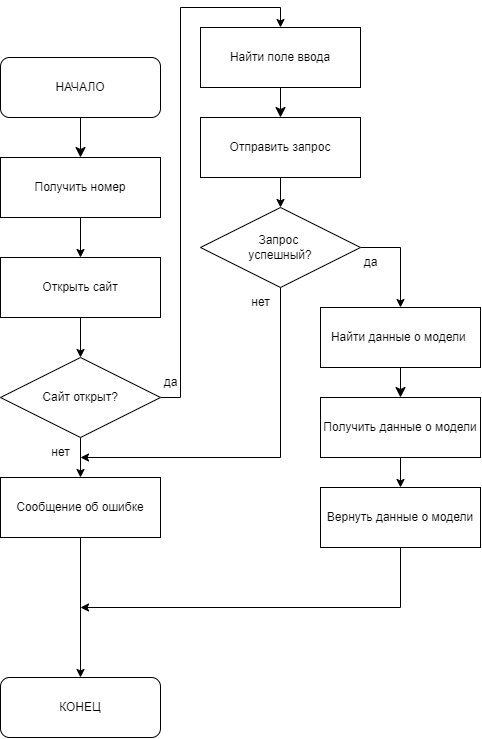
\includegraphics[width=0.5\textwidth]{search_alg}
	\caption{Алгоритм работы компонента для поиска модели}
	\label{f:search_alg}
\end{figure}



\subsubsection{Распознование номера автомобиля}

В этом разделе будет описан компонент, который используется для распознавания номерных знаков автомобиля, его алгоритм и функции. Рвссматриваются модели, которые он использует в процессе своей работы.

\paragraph{Обнаружение положения номерного знака}
Для обнаружения положения номерного знака используется предобученная модель model-resnet.tflite с архитектурой ResNet-50. Она предназначена для выявления границ номерного знака и выделение его области. ResNet-50 выбрана благодаря ее способности эффективно извлекать признаки из изображений и обучаться на больших объемах данных \refref{ref:res-net}. 

ResNet50 состоит из четырех ключевых модулей: сверточные слои, блок идентификации, сверточный блок и полностью связанные слои. Сверточные слои занимаются извлечением признаков из изображений, таких как края, текстуры и формы. Блок идентификации и сверточный блок обрабатывают и преобразовывают эти признаки. В завершение, полностью связанные слои отвечают за финальную классификацию \refref{ref:res-net}.

Сверточные слои ResNet50 состоят из нескольких сверточных блоков, сопровождаемых пакетной нормализацией и активацией. Они извлекают особенности из входных изображений и передают их дальше для анализа. Далее следуют слои объединения, которые уменьшают размеры карт признаков, сохраняя важные детали \refref{ref:res-net}.

Блок идентификации и сверточный блок - это основные строительные блоки ResNet50. Он передает входные данные через ряд сверточных слоев и добавляет к ним остаточные данные. Это позволяет сети изучать функции, оставшиеся после извлечения признаков. Сверточный блок аналогичен блоку идентификации, но использует сверточные слои 1x1 для уменьшения размерности перед основным сверточным слоем 3x3 \refref{ref:res-net}.

Полностью связанные слои выполняют окончательную классификацию. Выходные данные последнего полностью связанного слоя поступают на функцию активации softmax для получения вероятностей классов.

Графическое излбражение структуры представлено на рисунке~\ref{f:res_net}.
\begin{figure}[ht]
	\centering
	\vspace{\toppaddingoffigure}
	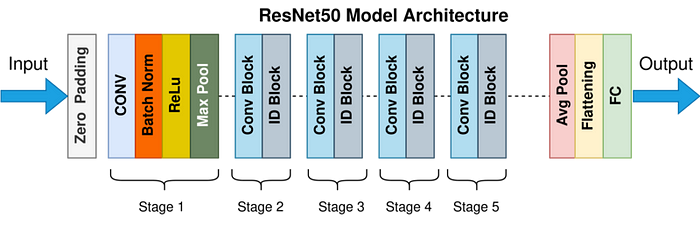
\includegraphics[width=0.7\textwidth]{res_net}
	\caption{Архитектура ResNet-50}
	\label{f:res_net}
\end{figure}



50-уровневая архитектура ResNet включает в себя следующие элементы:

\begin{itemize}
    \item свертка ядра 7 × 7 наряду с 64 другими ядрами с шагом в 2 размера;
    \item максимальный уровень объединения с шагом в 2 размера;
    \item 9 слоев- свертка ядра размером 3 × 3,64, другой с 1 × 1,64 ядрами и третий с 1 × 1256 ядрами. Эти 3 слоя повторяются 3 раза;
    \item 12 слоев с 1 × 1128 ядрами, 3 × 3128 ядрами и 1 × 1512 ядрами, повторяется 4 раза;
    \item 18 слоев с ядрами 1 × 1256 и 2 ядрами 3 × 3,256 и 1 × 1,1024, повторяется 6 раз;
    \item 9 слоев с ядрами 1 × 1512, 3 × 3512 и 1 × 12048 повторяются 3 раза;
    \item создание среднего пула, за которым следует полностью подключенный уровень с 1000 узлами, с использованием функции активации softmax.
\end{itemize}

Тестирование модели показало достаточно хороший уровень точности. Результаты тестирования представлены на рисунке~\ref{f:test1-res-net}.
\begin{figure}[ht]
	\centering
	\vspace{\toppaddingoffigure}
	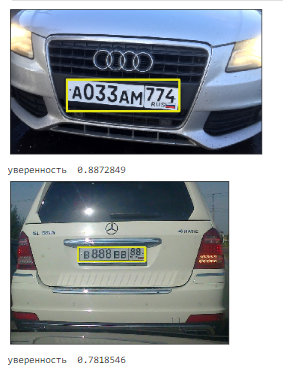
\includegraphics[width=0.3\textwidth]{test1-res-net}
	\caption{Тестирование модели}
	\label{f:test1-res-net}
\end{figure}


\paragraph{Определение номера автомобиля}

Для определения номера автомобиля используется предобученная модель model-nomer.tflite. Данная модель предназначена для определения текста на номерном знаке. фрагмент изображения с номерным знаком поступает от модели, описанной выше. Модель представляет собой комбинацю сверточной нейронной сети (CNN), рекуррентной нейронной сети долгой краткосрочной памяти (LSTM) и функции свертки по времени (CTC) для распознавания текста на изображениях. CNN используется для извлечения признаков из изображения номерного знака, LSTM преобразует эти признаки в последовательность символов, а CTC используется для выравнивания последовательности символов с фактическим текстом номера \refref{ref:cnn-lstm}.

Структура модели представлена на рисунке~\ref{f:cnn-lstm}.

\begin{figure}[h!]
	\centering
	\vspace{\toppaddingoffigure}
	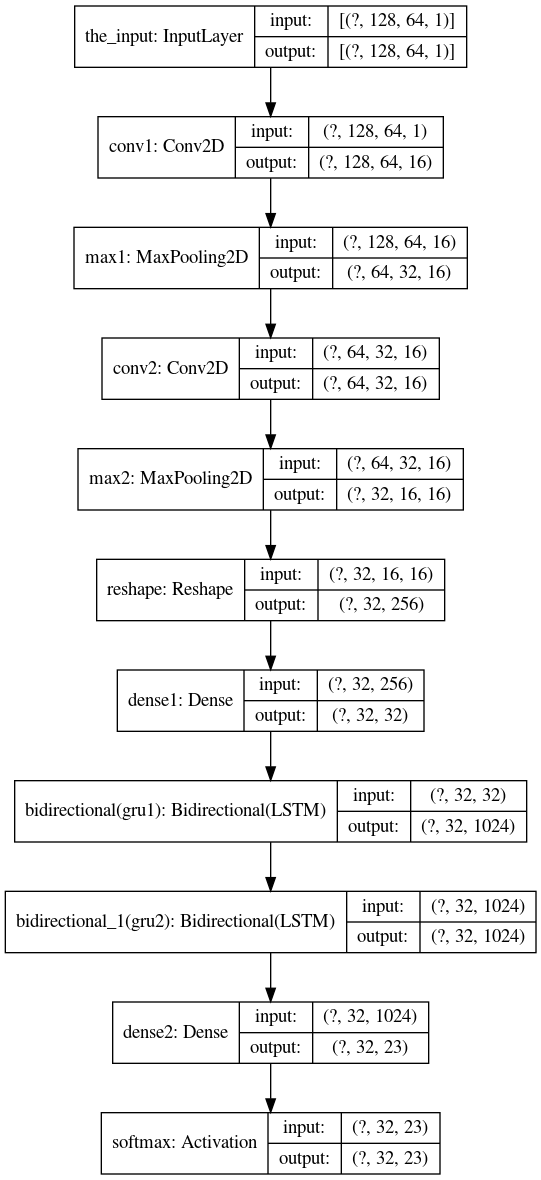
\includegraphics[width=0.4\textwidth]{cnn-lstm}
	\caption{Структура модели}
	\label{f:cnn-lstm}
\end{figure}

Результаты тестирования представлены на рисунке~\ref{f:test-cnn-lstm}.

\begin{figure}[h!]
	\centering
	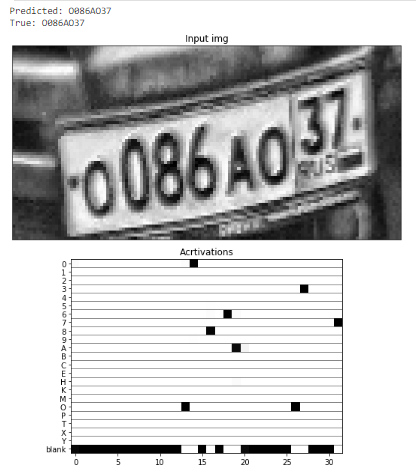
\includegraphics[width=0.4\textwidth]{test-cnn-lstm}
	\caption{Результаты тестирования}
	\label{f:test-cnn-lstm}
\end{figure}

\newpage

\paragraph{Алгоритм компонента}

К функциям компонента относятся следующие пункты:
\begin{itemize}
    \item загрузка и разбиение входного видео на кадры;
    \item выбор отдельного кадра;
    \item распознавание номера автомобиля на получившимся изображении.
\end{itemize}

Алгоритмы работы представлены на рисунках~\ref{f:nomer-alg-main}-~\ref{f:nomer-alg-recognize}.

\begin{figure}[h!]
	\centering
	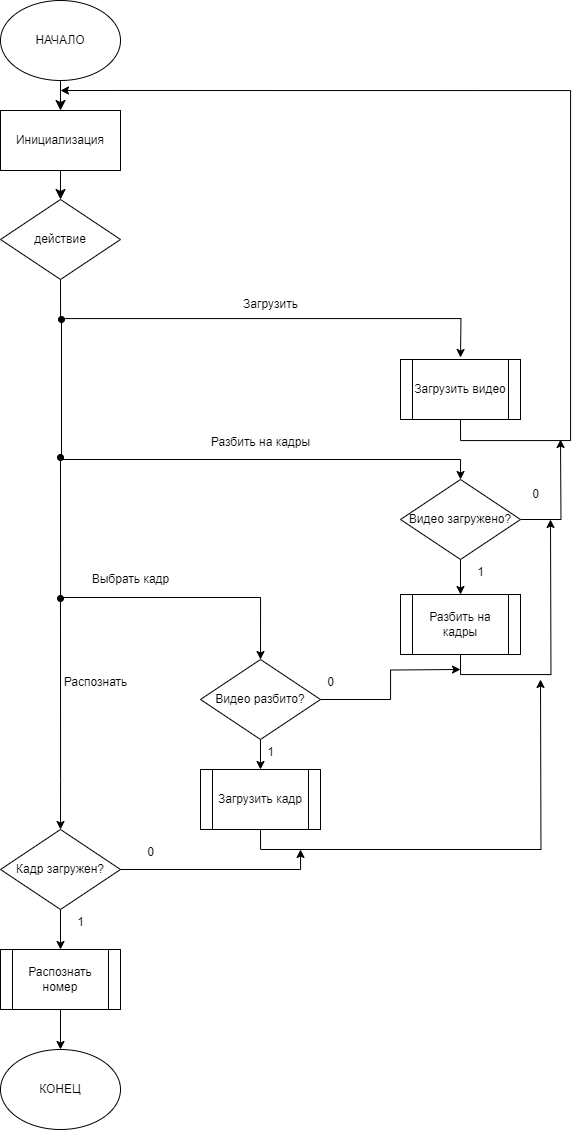
\includegraphics[width=0.6\textwidth]{nomer-alg-main}
	\caption{Схема алгоритма компонента распознавания номера}
	\label{f:nomer-alg-main}
\end{figure}

\newpage
\begin{figure}[h!]
	\centering
	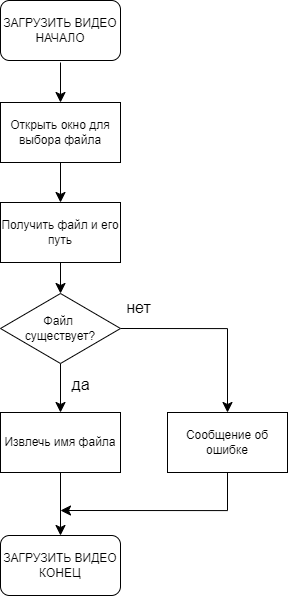
\includegraphics[width=0.22\textwidth]{nomer-alg-load}
	\caption{Схема алгоритма загрузки видео}
	\label{f:nomer-alg-load}
\end{figure}

\begin{figure}[h!]
	\centering
	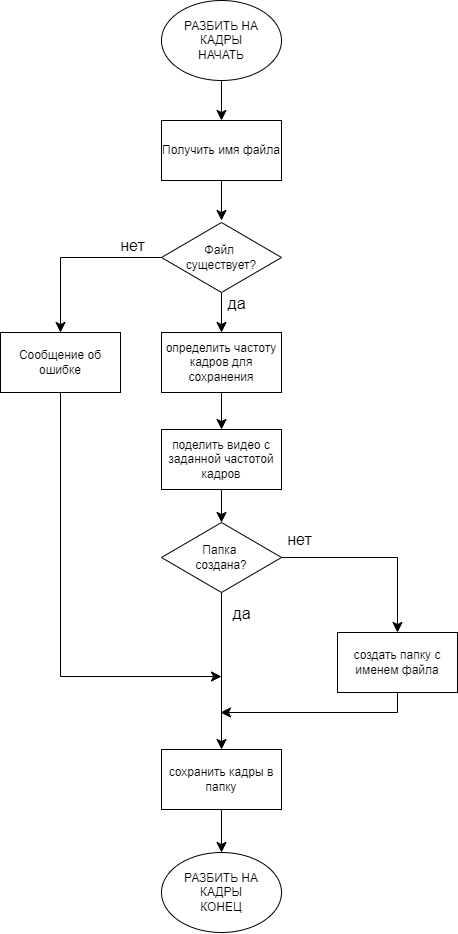
\includegraphics[width=0.35\textwidth]{nomer-alg-split}
	\caption{Схема алгоритма разбиения видео на кадры}
	\label{f:nomer-alg-split}
\end{figure}

\newpage

\begin{figure}[h!]
	\centering
	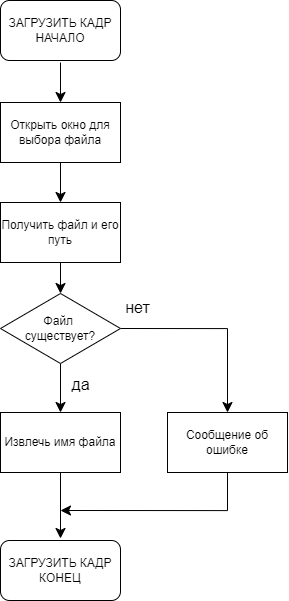
\includegraphics[width=0.22\textwidth]{nomer-alg-choose}
	\caption{Схема алгоритма выбора одного из кадров}
	\label{f:nomer-alg-choose}
\end{figure}

\begin{figure}[h!]
	\centering
	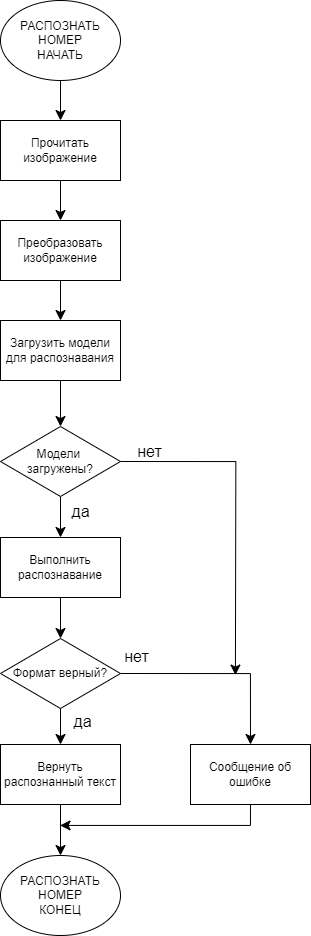
\includegraphics[width=0.25\textwidth]{nomer-alg-recognize}
	\caption{Схема алгоритма распознавания номера}
	\label{f:nomer-alg-recognize}
\end{figure}

\newpage
\section*{Выводы}

В этом разделе было рассмотрено описание модуля для сбора данных, был рассмотрен процесс разработки компонентов, входящих в модуль, а также их функции и особенности.